%!TEX TS-program = xelatex
\documentclass[12pt, a4paper]{article}  

\usepackage{etex} % расширение классического tex в частности позволяет подгружать гораздо больше пакетов, чем мы и займёмся далее

%%%%%%%%%% Математика %%%%%%%%%%
\usepackage{amsmath,amsfonts,amssymb,amsthm,mathtools} 
%\mathtoolsset{showonlyrefs=true}  % Показывать номера только у тех формул, на которые есть \eqref{} в тексте.
%\usepackage{leqno} % Нумерация формул слева


%%%%%%%%%%%%%%%%%%%%%%%% Шрифты %%%%%%%%%%%%%%%%%%%%%%%%%%%%%%%%%
\usepackage{fontspec}         % пакет для подгрузки шрифтов
\setmainfont{Arial}   % задаёт основной шрифт документа

\defaultfontfeatures{Mapping=tex-text}

% why do we need \newfontfamily:
% http://tex.stackexchange.com/questions/91507/
\newfontfamily{\cyrillicfonttt}{Arial}
\newfontfamily{\cyrillicfont}{Arial}
\newfontfamily{\cyrillicfontsf}{Arial}

\usepackage{unicode-math}     % пакет для установки математического шрифта
\setmathfont{Asana Math}      % шрифт для математики
% \setmathfont[math-style=ISO]{Asana Math}
% Можно делать смену начертания с помощью разных стилей

% Конкретный символ из конкретного шрифта
% \setmathfont[range=\int]{Neo Euler}

\usepackage{polyglossia}      % Пакет, который позволяет подгружать русские буквы
\setdefaultlanguage{russian}  % Основной язык документа
\setotherlanguage{english}    % Второстепенный язык документа


%%%%%%%%%% Работа с картинками %%%%%%%%%
\usepackage{graphicx}                  % Для вставки рисунков
\usepackage{graphics}
\graphicspath{{images/}{pictures/}}    % можно указать папки с картинками
\usepackage{wrapfig}                   % Обтекание рисунков и таблиц текстом
\usepackage{subfigure}                 % для создания нескольких рисунков внутри одного


%%%%%%%%%% Работа с таблицами %%%%%%%%%%
\usepackage{tabularx}            % новые типы колонок
\usepackage{tabulary}            % и ещё новые типы колонок
\usepackage{array}               % Дополнительная работа с таблицами
\usepackage{longtable}           % Длинные таблицы
\usepackage{multirow}            % Слияние строк в таблице
\usepackage{float}               % возможность позиционировать объекты в нужном месте
\usepackage{booktabs}            % таблицы как в книгах!
\renewcommand{\arraystretch}{1.3} % больше расстояние между строками

% Заповеди из документации к booktabs:
% 1. Будь проще! Глазам должно быть комфортно
% 2. Не используйте вертикальные линни
% 3. Не используйте двойные линии. Как правило, достаточно трёх горизонтальных линий
% 4. Единицы измерения - в шапку таблицы
% 5. Не сокращайте .1 вместо 0.1
% 6. Повторяющееся значение повторяйте, а не говорите "то же"
% 7. Есть сомнения? Выравнивай по левому краю!

%%%%%%%%%% Графика и рисование %%%%%%%%%%
\usepackage{tikz, pgfplots}  % язык для рисования графики из latex'a
\usepackage{amscd}                  %Пакеты для рисования
\usepackage[matrix,arrow,curve]{xy} %комунитативных диаграмм



\title{Графика в LaTeX, TikZ}
\date{\today}

\begin{document} % конец преамбулы, начало документа

\section{Внутренние средства для графики в \LaTeX{} или как не надо делать!}


\begin{center}
\begin{picture}(200,100)
\put(50,50){\oval(50,100)}
\put(150,50){\oval(50,100)}
\put(50,80){\circle*{2}}
\put(43,80){\footnotesize{1}}
\put(50,60){\circle*{2}}
\put(43,60){\footnotesize{2}}
\put(50,40){\circle*{2}}
\put(43,40){\footnotesize{3}}
\put(50,20){\circle*{2}}
\put(43,20){\footnotesize{4}}
\put(150,80){\circle*{2}}
\put(153,80){\footnotesize{5}}
\put(150,60){\circle*{2}}
\put(153,60){\footnotesize{11}}
\put(150,40){\circle*{2}}
\put(153,40){\footnotesize{12}}
\put(150,20){\circle*{2}}
\put(153,20){\footnotesize{17}}
\put(53,80){\vector(1,0){94}}
\put(147,80){\vector(-1,0){94}}
\put(53,60){\vector(1,0){94}}
\put(147,60){\vector(-1,0){94}}
\put(53,40){\vector(1,0){94}}
\put(147,40){\vector(-1,0){94}}
\put(53,20){\vector(1,0){94}}
\put(147,20){\vector(-1,0){94}}
\end{picture}
\end{center}

\begin{figure}[h!]
\begin{center}
\[ \xymatrix{
(1,1) \ar[r] &  (1,2) \ar[ld]  &  (1,3) \ar[r]  & (1,4) \ar[ld]  & (1,5)  \ar[r] & \dots  \\
(2,1) \ar[d] & (2,2) \ar[ru]  & (2,3) \ar[ld]  & (2,4) \ar[ur] & (2,5) &  \dots\\
(3,1) \ar[ru] & (3,2) \ar[ld] & (3,3) \ar[ur] & (3,4) & (3,5)  & \dots \\
(4,1) \ar[d] & (4,2) \ar[ur] & (4,3) & (4,4) & (4,5)  & \dots \\
(5,1) \ar[ur] & (5,2) & (5,3) & (5,4) & (5,5)  & \dots \\
\dots & \dots & \dots & \dots & \dots  }
\]
\caption{Нумерация элементов в множестве пар натуральных чисел $\mathbb{N}^2$}\label{n^2}
\end{center}
\end{figure}


\newpage 

\section{Великий и могучий Tikz}
\subsection{ Основные команды} 


% Никогда не забывать в конце каждой строки ставить ;
% Tikz очень капризен по отношению к этому!

\begin{tikzpicture}
% \draw[red, dashed, thick] (0,1) -- (2,1) (0,2) -- (2,2);
% \draw[->] (0,1) -- (-1,1);
% \draw[blue,fill=yellow](2,2) circle [radius = 0.5];
\end{tikzpicture}

\vspace{1cm}

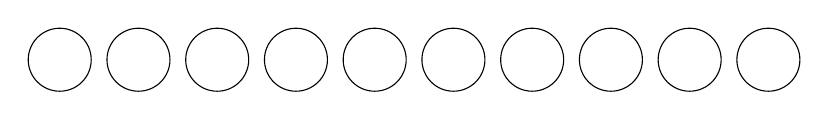
\begin{tikzpicture}
\foreach \x in {0,...,9} 
  \draw (\x,0) circle (0.4);
\end{tikzpicture}

\vspace{1cm}

% \draw [domain=<xmin>:<xmax>] plot (\x, {function})

\begin{tikzpicture}
% \draw [help lines] (-2,0) grid (2,4); 
% \draw [->] (-2.2,0) -- (2.2,0); 
% \draw [->] (0,0) -- (0,4.2); 
% \draw [green, thick, domain=-2:2] plot (\x, {4-\x*\x}); 
% \draw [domain=-2:2, samples=50] plot (\x, {1+cos(pi*\x r});
\end{tikzpicture}


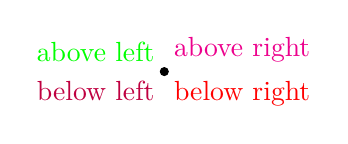
\begin{tikzpicture}[scale=2]
\draw[fill] (0.5,0.75) circle [radius=0.025];
\node [below right, red] at (0.5,0.75) {below right};
\node [above left, green] at (0.5,0.75) {above left};
\node [below left, purple] at (0.5,0.75) {below left};
\node [above right, magenta] at (0.5,0.75) {above right};
\end{tikzpicture}
% измнение scale не изменяет размер текста


\subsection{Tikztempaltes и их редактирование}

% \begin{figure}[h]
% \begin{center}

% \end{center}
% \caption{ }
% \end{figure}

\subsection{Geogebra}

% Нарисовать что-нибудь рандомное!




\end{document} % конец документа